\chapter{Motivation and Background of Stable Multithreading (\smt)}
\label{sec:smt-motivation}

This chapter first analyzes why multithreaded programs are so
difficult to get right (\S\ref{sec:smt-why}), and then introduces
\smt, our new approach that can greatly reduce the number of schedules for all
inputs, making multithreaded programs much easier to get right
(\S\ref{sec:smt-potential}). \smt is not the only technique to reduce the number
of schedules, and previously researchers have proposed a complementary technique
called Dterministic Multithreading (\dmt) that reduces the number of schedules
for each input, so this chapter also compares \smt with \dmt.

\section{Why Are Multithreaded Programs So Hard to Get Right?}
\label{sec:smt-why}

\begin{figure*}[t]
\begin{center}
\subfloat[{\em
Traditional.}]{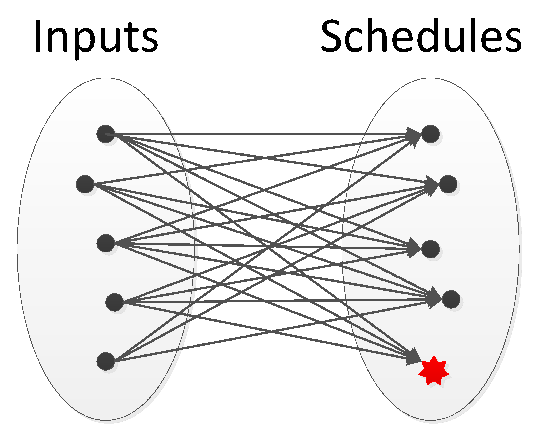
\includegraphics[width=.23\linewidth]{figures/nondet}
  \label{fig:nondet}}
\subfloat[{\em
Deterministic.}]{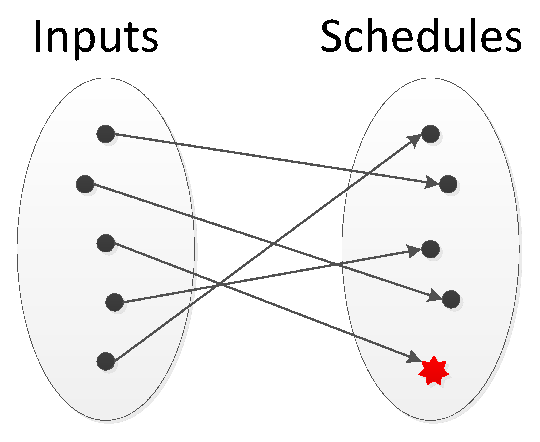
\includegraphics[width=.23\linewidth]{figures/dmt}
  \label{fig:dmt}}
\subfloat[{\em Stable
(deterministic).}]{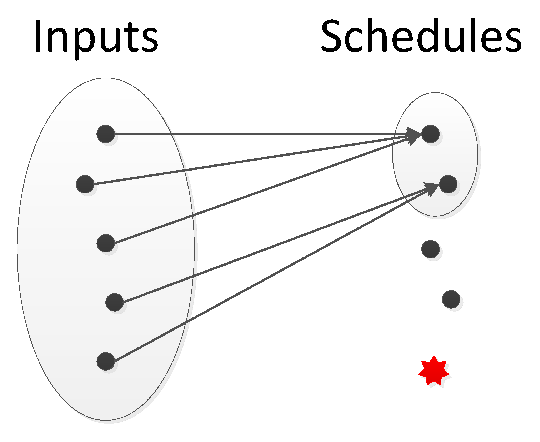
\includegraphics[width=.23\linewidth]{figures/smt}
  \label{fig:smt}}
\subfloat[{\em Stable
(nondeterministic).}]{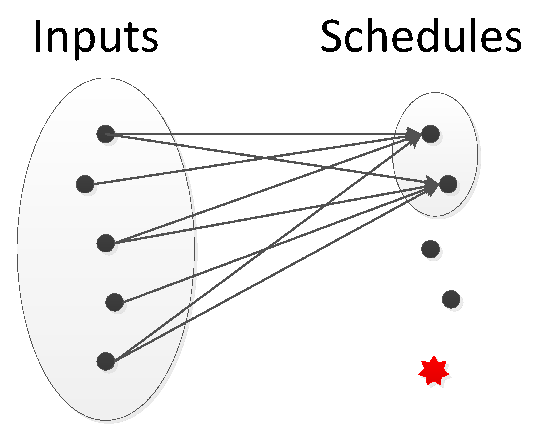
\includegraphics[width=.23\linewidth]{figures/smtn}
  \label{fig:smtn}}
\vspace{-.05in}
\caption{Different multithreading approaches. Red stars represent buggy
schedules.  Traditional multithreading (\subref*{fig:nondet}) is a conceptual
many-to-many mapping where one input may execute under many schedules because of
nondeterminism, and many inputs may execute under one schedule because a
schedule fixes the order of the communication operations but allows the local
computations to operate on any input data.  \dmt (\subref*{fig:dmt}) may map
each input to an arbitrary schedule, reducing programs' robustness on input
perturbations.  \smt (\subref*{fig:smt} and \subref*{fig:smtn}) reduces the
total set of schedules for all inputs (represented by the shrunk ellipses),
increasing robustness and improving reliability. \smt and \dmt are
complementary: a \smt system can be deterministic (\subref*{fig:smt}) or
nondeterministic (\subref*{fig:smtn}).}
\vspace{-.2in}
\end{center}
\end{figure*}

This section starts with preliminaries, and then reveals the key reason that
makes multithreading so difficult to get right is: a multithreaded program has
too many possible schedules for all inputs at runtime.

\subsection{Preliminaries: Inputs, Schedules, and Buggy Schedules}

To ease discussion, we use \emph{input} to broadly refer to the data a
program reads from its execution environment, including not only the data
read from files and sockets, but also command line arguments, return
values of external functions such as \vv{gettimeofday}, and any external data
that can affect program execution.  We use \emph{schedule} to broadly refer to
the (partially or totally) ordered set of communication operations in a
multithreaded execution, including synchronizations (\eg, \vv{lock} and
\vv{unlock} operations) and shared memory accesses (\eg, \vv{load} and
\vv{store} instructions to shared memory). Of all the schedules, most run
fine, but some trigger concurrency errors, causing program crashes,
wrong outputs, security breaches, and other failures. Consider the toy program
below: \lgrindfile{code/sync-bug.cpp} \noindent The schedule in which thread 2
gets the lock before thread 1 causes a dereference-of-NULL failure.  Consider
another example.  The toy program below has data races on \vv{balance}:
\lgrindfile{code/race-bug.cpp} \noindent The schedule with the statements
executed in the order shown corrupts \vv{balance}. We call the schedules that
trigger concurrency errors \emph{buggy schedules}.  Strictly speaking, the
errors are in the programs, triggered by a combination of inputs and schedules. 
However, typical concurrency errors, such as most errors appeared in previous
studies~\cite{lu:concurrency-bugs,con:hotpar12}, depend much more on the
schedules than the inputs (\eg, once the schedule is fixed, the bug
occurs for all inputs allowed by the schedule).  Thus, recent research on
testing multithreaded programs (\eg,~\cite{musuvathi:chess:osdi08}) is
focused on effectively testing schedules to find the buggy ones.

\subsection{Key Reason: Too Many Schedules For All Inputs}

A typical multithreaded program has an enormous number of schedules.  For
a single input, the number of schedules is asymptotically exponential in
the schedule length.  For instance, given $m$ threads each competing for a
lock $k$ times, each order of lock acquisitions forms a schedule, easily
yielding $\frac{(mk)!}{(k!)^m} \ge (m!)^k$ total schedules---a number
exponential in both $m$ and $k$. Aggregated over all inputs, the number of
schedules is even greater. Figure~\ref{fig:nondet} depicts the traditional
multithreading approach. Conceptually, traiditional multithreading runtimes
(\eg, Pthreads) maintain a many-to-many mapping from inputs to schedules, where
one input may execute under many schedules depending on hardware timings and OS
scheduling, and many inputs may execute under one schedule because a schedule
fixes the order of the communication operations but allows the local
computations to operate on any input data.

Finding a few buggy schedules in these exponentially many schedules raises
a series of ``needle-in-a-haystack" challenges on understanding, testing,
analyzing, and verification of multithreaded programs. For instance, when facing
these excessive schedules, developers' understanding are prone to mistakes, and
we have seen tons of concurrency bug reports sent to the email lists of
real-world software. Various forms of testing tools suffer, too.  Stress testing
is a common method for (indirectly) testing schedules, but it often redundantly
tests the same schedules while missing others. To mitigate redundant testing
effort, recent advanced testing tools (\eg,~\cite{musuvathi:chess:osdi08,
modist:nsdi09, dbug:ssv10, demeter:sosp11}) can systematically test schedules,
and these tools have included several remarkable reduction algorithms
(\eg,~\cite{flanagan:dynamicpo, demeter:sosp11}) to avoid testing the same
schedules and improve schedule coverage. Recent advanced program
analysis and verification tools (\eg,~\cite{demeter:sosp11}) also make notable
attempts to increase the number of checked schedules based on these reduction
algorithms. All these advanced tools have effectively found new harmful
concurrency bugs in real-world software. Unfortunately, despite of these great
effort, these tools still can not cover more than a tiny fraction of all
exponentially many schedules, and concurency bugs within an unchecked schedule
can show up in production runs and lead to critical failures and
vulnerabilities. Therefore, we argue that the exponentially many schedules for
all inputs is the key reason that causes multithreaded programs extremely
difficult to get right.


\section{Shrinking the Haystack with Stable Multithreading}
\label{sec:smt-potential}

\begin{table*}[t]
\centering
\small
\begin{tabular}{lll}
{\bf Program} & {\bf Purpose } & {\bf Constraints on inputs sharing schedules}
\\ \hline

\apache & Web server               & For a group of typical HTTP GET requests,
same cache status \\

\pbzip  & Compression              & Same number of threads \\

\aget   &  File download           & Same number of threads, similar file sizes 
\\

\barnes & N-body simulation        & Same number of threads, same values of two
configuration variables \\

\fft    & Fast Fourier transform   & Same number of threads \\

\luc    & Matrix decomposition     & Same number of threads, similar sizes of
matrices and blocks \\

\blackscholes & Option pricing     & Same number of threads, number of options
no less than number of threads    \\

\swaptions &  Swaption pricing     & Same number of threads, number of swaptions
no less than number of threads   \\

\end{tabular}
\vspace{-.05in}
\caption{{\em Constraints on inputs sharing the same equivalent class of
    schedules}.  For each program, one schedule out of the class
  suffices to process any input satisfying the constraints in the
  third column under typical setups (\eg, no system call failures or signals). 
We describe how to compute such constraints in \S\ref{sec:build}.}
\label{tab:sched-constraints}
\vspace{-.15in}
\end{table*}

To reduce the number of schedules and make multithreading easier to get right,
we investigated a central research question: \emph{are all the exponentially
many schedules necessary}?  A schedule is necessary if it is the only one
that can (1) process specific inputs or (2) yield good performance under
specific scenarios. Removing unnecessary schedules from the haystack would
make the needles easier to find.

We investigated this question on a diverse set of popular multithreaded
programs, ranging from server programs such as \apache, to desktop utilities
such as parallel compression utility \pbzip, to parallel implementations of
computation-intensive algorithms such as FFT.  These programs use diverse
synchronization primitives such as mutex locks, semaphores, condition variables,
and barriers.  Our investigation reveals the following two insights.

First, for many programs, a wide range of inputs share the same equivalent
class of schedules.  Thus, one schedule out of the class suffices to
process the entire input range.  Intuitively, an input often contains two
types of data: (1) metadata that controls the communication of the
execution, such as the number of threads to spawn; and (2) computational
data that the threads locally compute on.  A schedule requires the input
metadata to have certain values, but it allows the computational data to vary.
That is, it can process any input that has the same metadata.  For instance,
consider the aforementioned \pbzip which splits an input file
among multiple threads, each compressing one file block.  The
communication, \ie, which thread gets which file block, is independent of
the thread-local compression. Under a typical setup (\eg, no \vv{read}
failures or signals), for each different number of threads set by a user, \pbzip
can use two schedules (one if the file can be evenly divided by the number of
threads and another otherwise) to compress any file, regardless of the file
data.

This loose coupling of inputs and schedules is not unique to \pbzip; many
other programs also exhibit this property.
Table~\ref{tab:sched-constraints} shows a sample of our findings.  The
programs shown include three real-world programs, \apache, \pbzip, and
\aget (a parallel file download utility) and five implementations of
computation-intensive algorithms from two widely used benchmark suites,
Stanford's \splash and Princeton's \parsec. (We will describe
how to compute the constraints that a schedule places on the inputs in
Chapter~\ref{sec:tern}.)

Second, the overhead of enforcing a schedule on different inputs is often low.
Presumably, the exponentially many schedules allow the
runtime system to react to various timing factors and select an
efficient schedule.  However, results from the \smt systems we built
invalidated this presumption.  With carefully designed schedule
representations (Chapter~\ref{sec:peregrine}), our systems incurred less than
15\%
overhead enforcing schedules on different inputs for most evaluated programs.
Relevant systems (\eg,~\cite{kendo:asplos09, determinator:osdi10} also show that
carefully enforcing schedules can achieve only modest overhead. Afterall,
considering the reliability and security benefits introduced by \smt, We believe
this moderate overhead is worthwhile.

Leveraging these two insights, we have invented Stable Multithreading (or \smt),
a new multithreading approach that reuses each schedule on a wide range of
inputs, mapping all inputs to a dramatically reduced set of schedules.
By vastly shrinking the haystack, it addresses all the needle-in-a-haystack
challenges at once, making multithreaded programs much easier to understand,
test, analyze, and verify.

\subsection{Benefits}

By vastly reducing the set of schedules, \smt brings numerous reliability
and security benefits to multithreading.  We describe several:

\para{Understanding.} Developers now only need to focus on understanding a much
smaller set of schedules, which can greatly reduce their burden. Developers can
also save much time on checking inputs, because \smt stabilizes program
behaviors on a class of inputs that can be run with the same schedule, then
developers' understanding on the program behavior of one input can be applied to
all inputs within this class.

\para{Testing.} \smt automatically
increases the coverage of schedule testing tools, with coverage
defined as the ratio of tested schedules over all schedules.
For instance, consider \pbzip again which needs only two
schedules for each different number of threads under typical setups.  Testing 32
schedules effectively covers from 1 to 16 threads.  Given that (1) \pbzip
achieves peak performance when the number of threads is identical or close to
the number of cores and (2) a typical machine has up to 16 cores, 32 tested
schedules can practically cover most schedules executed in the field.

\para{Debugging.} Reproducing a bug now does not require the exact input,
as long as the original and the altered inputs map to the same schedule.
It does not require the exact program either, as long as the changes to
the program do not affect the schedule.  Users may remove private
information such as credit card numbers from their bug reports. Developers
may reproduce the bugs in different environments or add \vv{printf}
statements. We will describe this benefit in more details in \S\ref{sec:tern}.

\para{Analyzing and verifying programs.} Static analysis can now focus
only on the set of schedules enforced in the field, gaining
precision.  Dynamic analysis enjoys the same benefits as testing.  Model
checking now only need to check drastically fewer schedules, mitigating the
so-called ``state explosion'' problem~\cite{clarke:ModelChecking}. We have
integrated our \parrot~\cite{parrot:sosp13} system with an open source model
checker called DBug~\cite{dbug:spin11}, and \parrot significantly increases the
number of programs that \dbug can exhaust searching schedules under our
evaluation settings. More details will be given in Chapter~\ref{sec:parrot}.
Interactive theorem proving, a popular technique on ensuring strong security and
reliability properties in software, becomes much easier, too, because verifiers
need to prove theorems only on the set of schedules enforced in the field.  We
will describe these benefits in more details in Chapter~\ref{sec:peregrine}.

\para{Avoiding errors at runtime.}  Programs can also adaptively learn correct
schedules in the field, then reuse them on future inputs to avoid unknown,
potentially buggy schedules.  We will describe this benefit in more
details in Chapter~\ref{sec:tern}.

\subsection{Caveats}

\smt is certainly not for every multithreaded program.  It works well with
programs whose schedules are loosely coupled with inputs, but there are also
other programs.  For instance, a program may decide to spawn
threads or invoke synchronizations based on intricate conditions involving many
bits in the input. The parallel \vv{grep}-like utility \pfscan is an example. 
It
searches for a keyword in a set of files using multiple threads, and for each
match, it grabs a lock to increment a counter.  A schedule computed on one set
of files is unlikely to suit another. To increase the input range each schedule
covers, developers can exclude the operations on this lock from the schedule
using annotations.


% \smt provides robustness and stability on small input and program
% perturbations when they do not affect schedules.  However, there
% is still room to improve.  For instance, when developers change their
% programs by adding synchronizations, it may be more efficient to
% update previously computed schedules rather than to recompute from
% scratch. We leave this idea for future work.



\section{Determinism: Not as Good as Commonly Perceived} \label{sec:smt-dmt}

A multithreaded program is \emph{nondeterministic} because even with the same
program and input, different executions may still run into different schedules
and trigger different behaviors, depending on such factors as physical timings
and OS scheduling. For instance, the two toy programs in the previous subsection
do not always run into the bugs.  Except for the schedules described, the
other schedules lead to correct executions. This nondeterminism raises many
challenges, especially in testing and debugging.  Suppose an input can execute
under $n$ schedules. Testing $n-1$ schedules is not enough for complete
reliability because the single untested schedule may still be buggy.  An
execution in the field may hit this untested schedule and fail.  Debugging is
challenging, too. To reproduce a field failure for diagnosis, the exact input
alone is not enough. Developers must also manage to reconstruct the buggy
schedule out of $n$ possibilities.

To address the challenges raised by nondeterminism, researchers have dedicated
much effort and built several Deterministic MultiThreading (or \dmt) systems
that force a multithreaded program to always run the same schedule on the same
input.  This determinism does have value for reliability.  For instance, one
testing execution now validates all future executions on the same input, and 
reproducing a concurrency error now requires only the input.

However, \dmt only focuses on reducing the number schedules on each input, and it does not help much on reducing the number of schedules for all inputs of a multithreaded program.  We believe
the community has charged nondeterminism more than its share of the guilt
and overlooked the main culprit---a rather quantitative cause that
multithreaded programs simply have too many schedules.
We argue that, although determinism has value, its value
is smaller than commonly perceived: it is neither sufficient nor
necessary for reliability.

\para{Determinism $\centernot \implies$ reliability.} Determinism is a
narrow property: same input + same program = same behavior. It has no
jurisdiction if the input or program changes however slightly.  Yet, we
often expect a program to be robust or stable against slight program
changes or input perturbations.  For instance, adding a debug \v{printf}
should in principle not make the bug disappear.  Similarly, a single bit flip of
a file should usually not cause a compression utility to crash. Unfortunately,
determinism does not provide this stability and, if na\"{i}vely implemented,
even undermines it.

To illustrate, consider the system depicted in
Figure~\ref{fig:dmt} which maps each input to an arbitrary schedule. This
mapping is perfectly deterministic, but it destabilizes program
behaviors on multiple inputs.  A single bit flip may force a program to
discard a correct schedule and adventure into a vastly different, buggy
schedule. This instability is counterintuitive at least,
and raises new reliability challenges.  For instance, testing one input
provides little assurance on very similar inputs, despite that the differences
in input do not invalidate the tested schedule.  Debugging now requires
every bit of the bug-inducing input, including not only the data a user
typed, but also environment variables, shared libraries, \etc.  A
different user name?  Error report doesn't include credit card numbers?
The bug may never be reproduced, regardless of how many times developers
retry, because the schedule chosen by the deterministic system for the
altered input happens to be correct. Besides inputs, na\"{i}vely implemented
determinism can destabilize program behaviors on minor code changes, so adding a
debug \vv{printf} causes the bug to deterministically disappear.  Another
problem is that the number of all possible schedules remains enormous, so the
coverage of schedule testing tools remains low.

In practice, to mitigate these problems, researchers have to augment
determinism with other techniques.  To support debug \vv{printf}, some
propose to temporarily revert to nondeterministic
execution~\cite{dmp:asplos09}.  DMP~\cite{dmp:asplos09},
CoreDet~\cite{coredet:asplos10}, and Kendo~\cite{kendo:asplos09} change
schedules only if the inputs change low-level instructions executed.
Although better than mapping each input to an arbitrary schedule, they
still allow small input perturbations to destabilize schedules
unnecessarily when the perturbations change the low-level instructions
executed (\eg, one extra \vv{load} executed), observed in our
experiments~\cite{cui:tern:osdi10}.

\para{Reliability $\centernot \implies$ determinism.} Determinism
is a binary property: if an input maps to $n > 1$ schedules, executions on this
input may be nondeterministic, however small $n$ is.  Yet, a nondeterministic
system with a small set of total schedules can be made reliable easily. 
Consider an extreme case, the nondeterministic system depicted in
Figure~\ref{fig:smtn} which maps all inputs to at most two schedules.  In this
system, the challenges caused by nondeterminism (\S\ref{sec:nondet}) are
easy to solve.  For instance, to reproduce a field failure given an input,
developers can easily afford to search for one out of only two schedules.
To offer an analogy, a coin toss is nondeterministic, but humans have
no problem understanding and doing it because there are only two possible
outcomes.

\dmt is complementary to \smt. \smt aims to reduce the set of schedules for
\emph{all} inputs, whereas DMT aims to reduce the schedules for \emph{each}
input (down to one).  A \smt system may be either deterministic or
nondeterministic. Figure~\ref{fig:smt} and Figure~\ref{fig:smtn} depict two \smt
systems: the many-to-one mapping in Figure~\ref{fig:smt} is deterministic, while
the many-to-few mapping in Figure~\ref{fig:smtn} is nondeterministic.  A
many-to-few mapping improves performance because the runtime system can choose
an efficient schedule out of a few for an input based on current timing factors,
but it increases the efforts and resources needed for reliability.  Fortunately,
the choices of schedules are only a few (\eg, a small constant such as two), so
the challenges caused by nondeterminism are easy to solve. Our \tern, \peregrine, and \parrot systems and others' \dthreads~\cite{dthreads:sosp11} built subsequently to \tern combine \dmt with \smt (elaborated next section) to frequently reuse schedules on a wide range of inputs for stability. The following three chapters will present our three systems.
